% ****** Start of file apssamp.tex ******
%
%   This file is part of the APS files in the REVTeX 4.1 distribution.
%   Version 4.1r of REVTeX, August 2010
%
%   Copyright (c) 2009, 2010 The American Physical Society.
%
%   See the REVTeX 4 README file for restrictions and more information.
%
% TeX'ing this file requires that you have AMS-LaTeX 2.0 installed
% as well as the rest of the prerequisites for REVTeX 4.1
%
% See the REVTeX 4 README file
% It also requires running BibTeX. The commands are as follows:
%
%  1)  latex apssamp.tex
%  2)  bibtex apssamp
%  3)  latex apssamp.tex
%  4)  latex apssamp.tex
%
\documentclass[%
 reprint,
nofootinbib,
%superscriptaddress,
%groupedaddress,
%unsortedaddress,
%runinaddress,
%frontmatterverbose,
%preprint,
%showpacs,preprintnumbers,
%nofootinbib,
%nobibnotes,
%bibnotes,
aps,
%pra,
%prb,
%rmp,
%prstab,
%prstper,
%floatfix,
]{revtex4-1}

\usepackage[utf8]{inputenc}
\usepackage[english]{babel}
\usepackage{dsfont}
\usepackage{amsmath}
\usepackage{ mathrsfs }
\usepackage{amssymb}
\usepackage{graphicx}% Include figure files
\usepackage{dcolumn}% Align table columns on decimal point
\usepackage{bm}% bold math
\usepackage{amsmath}
\usepackage{varioref}
\usepackage{booktabs}
\usepackage[bottom]{footmisc}

\usepackage{physics}

\usepackage{algpseudocode}
\usepackage{listings}

\usepackage{booktabs}

\usepackage{tikz}

\newcommand{\RN}[1]{%
  \textup{\uppercase\expandafter{\romannumeral#1}}%
}


\newcolumntype{C}{>{$}c<{$}}
\AtBeginDocument{
\heavyrulewidth=.08em
\lightrulewidth=.05em
\cmidrulewidth=.03em
\belowrulesep=.65ex
\belowbottomsep=0pt
\aboverulesep=.4ex
\abovetopsep=0pt
\cmidrulesep=\doublerulesep
\cmidrulekern=.5em
\defaultaddspace=.5em
}

%\usepackage{hyperref}% add hypertext capabilities
%\usepackage[mathlines]{lineno}% Enable numbering of text and display math
%\linenumbers\relax % Commence numbering lines

%\usepackage[showframe,%Uncomment any one of the following lines to test
%%scale=0.7, marginratio={1:1, 2:3}, ignoreall,% default settings
%%text={7in,10in},centering,
%%margin=1.5in,
%%total={6.5in,8.75in}, top=1.2in, left=0.9in, includefoot,
%%height=10in,a5paper,hmargin={3cm,0.8in},
%]{geometry}

\begin{document}

%\preprint{APS/123-QED}

\title{The Ising Model}% Force line breaks with \\


\author{Ivar Svalheim Haugerud}\homepage{http://www.github.uio.no/ivarsh/FYS4150}

\affiliation{%
 Department of Physics, University of Oslo\\
}%


\date{\today}% It is always \today, today,
             %  but any date may be explicitly specified

\begin{abstract}
Metropolis, the Monte Carlo based algorithm, is used to study the phase transitions of the Ising model numerically in a two dimensional lattice with periodic boundary conditions. We start by reproducing analytical results for the $2\times 2$ lattice, making sure our algorithm is working. We then expand to a $20\times 20$ lattice, and study the equilibration time for different temperatures and initial conditions. We find that we approximately need $10^4$ MC cycles for reaching equilibrium, independent of initial condition. Counting the number of times each energy occurs we are able to find the probability distribution function without having to calculate it explicitly. For lower temperatures we find a much smaller variance compared to the higher temperatures. For fast computing the code is parallelized on four cores, making the code $3.6(2)$ times faster. The phase transition is studied in detail, and we find the critical temperature to be $2.2698(6)J/k_B$, when the analytical value is $ 2.2692J/k_B$, correct to the analytical one within uncertainties..
\end{abstract}
\maketitle


\section{Introduction}

The Ising model describes the magnetic properties of ferromagnetic materials. It is a simplified classical model, with quantized spin, where each spin is only allowed to interact with it's nearest neighbours in a fixed lattice. Even though the model is simple, many important physical properties can be derived from it. Studying the Ising model numerically has it's problems. Even though each particle only has two possible states, spin up or spin down, the total number of possible states will become very large, even for small systems. This means that we are limited in what properties we can calculate numerically, for example will the probability distribution function be impossible to calculate. This problem is solved by using the Monte Carlo based Metropolis algorithm. The Metropolis algorithm can be used to sample the probability distribution function of complicated systems. With this method we avoid the numerically toughest calculations while still simulating the system accurately and being able to calculate physical observables. Our results can be tested against theory, as the system is solved analytically by Lars Onsager \cite{onsager}.\\
In this article we begin by benchmarking our algorithm with analytical results for a $2\times 2$ lattice. We then increase the size of the system to a $20\times 20$ lattice, where we study the numerical path to equilibrium, the acceptance of states for different temperatures, and sample the probability distribution function for one temperature above, and one below, the  critical temperature. We then study the phase transition, and calculate the critical temperature by assuming a power law around the critical temperature.
\\
Understanding magnets is important fundamental research, and has many applications. Magnets are used in technology, industry, medicine and much more. Understanding their behaviour can therefore be exploited in new technology with important applications. Understanding the behaviour of magnets gives us fundamental insight within condensed matter.
\\
In this article we will start by going through the theory used, how the algorithm incorporates them, and how we use these algorithms to answer our questions. We go through the results we produce, and discuss the results and their implications, before concluding on our work.

\section{Theory}
\subsection{Statistical Mechanics}
When working on systems with many degrees of freedom we do not have the possibility to know the position and velocity of every particle, and if we did the calculations would be too demanding for interesting systems. Instead we model the system statistically, using probability models and microscopic physical laws. With this we are able to derive macroscopic properties, and understand the behaviour of many-particle systems.
The probability of observing a given state $i$ is
\begin{equation}
    P_i = \frac{1}{Z}e^{-E_i\beta}, \label{eq:prob}
\end{equation}
where $E_i$ is the energy of state $i$, and $\beta = 1/k_BT$, $k_B$ is Boltzmann's constant and $T$ is the temperature. We see that the system is more likely to be in the lower energy states, but with increasing temperatures this effect plays a smaller role. The exponential factor is called the Boltzmann factor. The variable $Z$ is the partition function of the system, and is defined as
\begin{equation}
    Z = \sum_{i}^{N}e^{-\beta E_i}, \label{eq:partifunc}
\end{equation}
where $N$ is the number of accessible states. The partition function plays the role as a normalization constant for the probabilities \eqref{eq:prob}, as well as containing many physical properties. The relationship between two probabilities is given by
\begin{equation}
  \frac{P(E_i)}{P(E_j)} = \frac{e^{-E_i/k_BT}/Z}{e^{-E_i/k_BT}/Z} = e^{(E_j-E_i)/k_BT} \label{eq:prob_rel}
\end{equation}

We can use the probability of measuring a given state \eqref{eq:prob} to calculate the expectation value of different physical properties of the system. For the Ising model we are interested in the magnetization $M$ and the energy $E$
\begin{align}
    \langle M \rangle &= \frac{1}{Z}\sum_{i=1}^{N}M_ie^{-E_i\beta} \label{eq:E}\\
    \langle E \rangle &= \frac{1}{Z}\sum_{i=1}^{N}E_ie^{-E_i\beta}, \label{eq:M}
\end{align}
Exactly the same can be done for $\langle M^2\rangle$ and $\langle E^2\rangle$, by squaring their respective quantity inside the sum.
From these results we can derive other physical properties as well. The heat capacity at a constant volume $C_V$, which describes the amount of energy needed to change the temperature, is given by
\begin{equation}
    C_V = \frac{1}{k_BT^2}\left( \langle E^2\rangle - \langle E \rangle^2\right) \label{eq:Cv}
\end{equation}
In the same fashion we can find the magnetic susceptibility, $\chi$, which tells us if the material is attracted into or repelled out of a magnetic field,
\begin{equation}
    \chi = \frac{1}{k_BT}\left( \langle M^2 \rangle - \langle M \rangle^2 \right) \label{eq:chi}
\end{equation}

For different thermal systems we have different thermodynamic potentials which will be minimized. For the system we will study the Helmholtz Free Energy $F$, defined as
\begin{equation}
    F = \langle E \rangle - TS,
\end{equation}
where $S$ is the entropy, will be minimized. The Helmholtz free energy of a system describes the fight between to important principles in physics; minimal energy and maximal entropy. When equilibrium is reached, for a given temperature, we are in a balance between the two properties, and the Helmholtz free energy is minimized.


In Statistical mechanics it is important to know the difference between the macro- and micro-state. The macro state refers to its macroscopic properties, such as its temperature, pressure, volume and density. For the Ising model the properties might be the magnetic susceptibility and the heat capacity, which we can easily probe in an experiment. The microstate is a specific microscopic configuration of the systems small constituent parts. Most of the time there are many different microstates which result in the same macrostate. And for an isolated system the equilibrium state is the one which has the largest amount of corresponding microstates.

\subsection{The Ising Model}
The Ising model is a model of ferromagnetic materials using statistical mechanics. The model uses quantized variables which represents the magnetic dipole moments of atomic spins. The spins can access two different states; spin up $\uparrow (+1)$ and spin down $\downarrow (-1)$. The position of each spin is confined to a lattice, which allows each spin to only interact with it's neighbour's. This is a simple model of a complicated system, but still gives us information about the system, as for example the critical temperature of the phase transition of the materials. The Hamilton of the Ising model is
\begin{equation}
    \hat{H} = -J\sum_{\langle k, l \rangle} S_kS_l, \label{eq:hamil}
\end{equation}
where $\langle k, l\rangle$ means summing over the nearest neighbours of every atom, $J$ is the coupling constant which denotes the strength of the interaction, and $S_k$ and $S_l$ is the spin of lattice point $k$ and $l$ respectively, and can have the values $\pm 1$. Two neighbouring spins will give a negative contribution to the energy if they are aligned the same direction, and a positive contribution if they are disaligned. In this model all of the interaction between the atoms is through the spins. When most of the spins align we have a ferromagnetic material, and when they disalign we have an anti-ferromagnetic material. Using a two dimensional grid each atom has four neighbours. The total energy of the system is found by summing over the energy for each lattice point, and counting each interaction only once.

From our model there are certain physical properties we want to calculate. One of these properties is the total energy of the system for a given macro-state. We can calculate this using the Hamiltonian \eqref{eq:hamil} and sum over every lattice point, and it's corresponding energy due to it's neighbours
\begin{equation}
    E = -J\sum_{\langle k, l \rangle} S_kS_l. \label{eq:energy}
\end{equation}
Another property is the total magnetization of our system $M$, which is calculated by summing over the spin in every lattice point and summing up the magnetic moment $S$
\begin{equation}
    M = \sum_{i}S_i.
\end{equation}

\subsection{The phase transition}
A phase transition results in abrupt changes macroscopic properties. The phase transition takes place as external parameters are changed, such as an increase the temperature, pressure, magnetic field, etc. The value needed of such an external parameter to induce a phase transition is called it's critical value.\\
It can be showed that the mean magnetization, for temperatures less than the critical temperature, follows
\begin{equation}
    \langle M \rangle \sim \left(T-T_c\right)^{\beta},
\end{equation}
where $\beta=1/8$ is called the critical exponent. One can find the same expression for the heat capacity as well as the magnetic susceptibility
\begin{align}
    C_V &\sim \abs{T_c-T}^{-\alpha} \label{CVALPHA}\\
    \chi &\sim \abs{T_c-T}^{-\gamma}, \label{CHIGAMMA}
\end{align}
with $\alpha = 0$ and $\gamma = -7/4$.\\
The phase transition changes the order of the system. To quantify this we will use the correlation length, $\xi$. The value of the correlation length is expected to approach the lattice distance $L$ as the temperature approaches the critical temperature. The behaviour of the correlation length close to the critical temperature is
\begin{equation}
    \xi = \abs{T_c-T}^{-\nu}.
\end{equation}
The correlation length for a finite lattice size $L$ can then be shown to be proportional to $L$. Using what we had earlier we get the following relations
\begin{align}
    \begin{split}
        \langle M \rangle &\propto L^{-\beta/\nu} \\
        C_V &\propto L^{\alpha/\nu} \\
        \chi &\propto L^{\gamma/\nu}
    \end{split}
\end{align}
Through so-called finite size scaling relations it is possible to relate the behavior at finite lattices with that of an infinitely large lattice. The critical temperature scales then as
\begin{equation}
  T_C(L=\infty) = T_C(L)-aL^{-1/\nu} \label{eq:noe}.
\end{equation}
Finding the value of $T_C(L=\infty)$ is done by finding the linear relationship of the critical temperature and the reciprocal lattice size, $L^{-1}$, in our data.
\subsection{Analytical results}\label{sec:analytic}
The Norwegian born chemists and physicists Lars Onsager was the first two solve the Ising model analytically in two dimensions for a general lattice size $L$ \cite{onsager}. He found that the critical temperature of the system is
\begin{equation}
  T_C = \frac{2J}{k_B\ln{\left(1+\sqrt{2}\right)}} \approx 2.26918..., \label{eq:Tc}
\end{equation}
where the numerical value of was found using $k=J=1$.
In our study we will compare our numerical results with the analytical ones for a $2\times 2$ system with periodic boundary conditions. The expectation values and the partition function can then be calculated through equations (\ref{eq:partifunc}, \ref{eq:E}, \ref{eq:M}). In the same manner one can find the expectation values of $E^2$ as well as $M^2$. We find that
\begin{align}
  Z &= 12 + 4\cosh{\left(8J\beta\right)} \\
  \langle E \rangle &= \frac{-32J\sinh{\left( 8J\beta \right)}}{Z}\\
  \langle E^2 \rangle &= \frac{256J^2\cosh{\left( 8J\beta \right)}}{Z}\\
  \langle \abs{M} \rangle &= 8\frac{2+e^{8J\beta}}{Z} \\
  \langle M^2 \rangle &= 32\frac{1+e^{8J\beta}}{Z}
\end{align}
With these analytical results we can compare our numerical results with theory. In addition we can calculate the heat capacity \eqref{eq:Cv} as well as the magnetic susceptibility \eqref{eq:chi}. If our results are correct for the $2\times 2$ system, we should get the correct results when increasing the lattice size as well.\\

\section{Algorithm}\label{sec:algorithms}
To simulate the Ising model we will use the Monte Carlo based Metropolis algorithm. The reason for using the Metropolis algorithm, is that we avoid having to calculate the probability distribution function (PDF). For our statistical mechanical system, the chance of observing the system in a given state is the Boltzmann factor \eqref{eq:prob}, which is normalized by the partition function \eqref{eq:partifunc}. To use the PDF we need the partition function.  To find the partition function we need to do heavy computations for every single possible state, which is numerically uneconomical. We will therefore use the Metropolis algorithm, which only uses ratios between probabilities, and we therefore do not need the partition function at all  \eqref{eq:partifunc}. The Metropolis algorithm works by creating a random initial state, and find it's energy $E_0$ and magnetization $M_0$. Then do the following in a loop:
\begin{itemize}
    \item Choose a random spin, and calculate the resulting change in energy if we were to flip this spin, $\Delta E$
    \item \begin{itemize}
        \item If $\Delta E \leq 0$ we accept the new configuration, and flip the spin.
        \item If $\Delta E > 0$ we only accept the new configuration if $e^{-\Delta E\beta}\geq r$, where $r$ is a random number between $0$ and $1$.
    \end{itemize}
    \item We update the expectation values we are interested in
\end{itemize}
When this loop has selected $L^2$ random spins, it is called a Monte Carlo cycle. The Monte Carlo part of the algorithm is the way we choose which spin to flip, and update the expectation values. The Metropolis part is the requirement for flipping a spin or not. The more Monte Carlo cycles we use the more precise our result will become. For each Monte Carlo cycle we will add the energy, energy squared, magnetization and magnetization squared, as well as the absolute value of the magnetization, to an array containing the sum of these values up until this state. After the algorithm is finished we calculate the expectation values for the quantities by dividing with the number of MC cycles.
\par
For a computer random numbers can never truly be random. The cycle of random numbers we use for $r$, and for finding the random spin to flip, follows a deterministic pattern, when given an initial seed. Since the random function will be called $L^2$ times the number of MC cycles, the number of calls will be very large. The maximal system we will run for is $200\times 200$, with $10^{6}$ MC cycles. This means that we will call the random function $5\times 10^{10}$ times, when including the equilibration time. For the algorithm to work we need to sample random numbers with a period of larger than $5\times 10^{10}$. Since we need a large period we will use the random number generator called Mersenne Twister, which has a period of $2^{19937}$. With this random number generator we have a period much larger than we will ever need, and is perfect for our system. Most other random number generators does not have such a large period, and it is therefore important that we use the Mersenne Twister.

\section{Method}
\subsection{Boundary conditions}
The number of particles in a real materials is on the order of Avogadro's number, $10^{23}$. In statistical mechanics we often let analytically solvable systems approach the thermodynamic limit, that is letting the number of particles go to infinity. Numerically we can never simulate a system of that size, the maximum value we will use is $200\times 200$. In the thermodynamic limit the number of particles goes to infinity, and therefore the boundary condition does not matter. To approximate a larger system we will use periodic boundary conditions. This way our system will not have any boundary as we are effectively projecting the two dimensional square lattice onto a sphere, as the upper atoms are in contact with the bottom row, and the same for the left and right side. With periodic boundary conditions every atom has four neighbours, and we are approximating the thermodynamic limit, as the boundaries play no role in the thermodynamic limit. \\
The periodic boundary condition is easily implemented in our program by introducing an index vector with the values $[L-1, 0, 1, 2, ..., L-2, L-1, 0]$. Every time we index the matrix containing the spins we will in instead index the index vector, and use the resulting value of the index-vector as the the spin-matrix-index. With this method we will make the algorithms more simple and avoid if-tests and other time consuming operations to account for the periodic boundary conditions.

\subsection{Efficiency}
For the two dimensional Ising model we only have $5$ possible values for $\Delta E$, and these can therefore be precalculated outside of the loop, to reduce the number of FLOPS. We will only have to calculate the five possible Boltzmann factors once for each temperature, this way we will avoid calling an exponential function $L^2$ times for each MC cycle, as this would be very time consuming. The possible values of change in energy is displayed in table \vref{table:1} for each possible case.

\begin{table}[]
\caption{The different possible changes in energy $\Delta E$ for different neighbours. This is shown to display that the change in energy can only have five possible values in a two dimensional lattice, when only interacting with the nearest neighbours. The position of the neighbouring spins does not matter for the change in energy.}
\label{table:1}
\begin{tabular}{@{}ccccc@{}}
\toprule
Initial state    & Final state        & Initial $E$ [J] & Final $E$ [J] & $\Delta E$ {[}J{]} \\ \midrule
$\begin{matrix}& \uparrow & \\ \uparrow & \uparrow & \uparrow \\ & \uparrow & \\ & & & \end{matrix}$         & $\begin{matrix}& \uparrow & \\ \uparrow & \downarrow & \uparrow \\ & \uparrow & \\ & & & \end{matrix}$ & -4 & 4 &     8                  \\
$\begin{matrix}& \downarrow & \\ \uparrow & \uparrow & \uparrow \\ & \uparrow & \\ & & & \end{matrix}$       & $\begin{matrix}& \downarrow & \\ \uparrow & \downarrow & \uparrow \\ & \uparrow & \\ & & & \end{matrix}$ & -2 &  2    & 4                  \\
$\begin{matrix}& \downarrow & \\ \downarrow & \uparrow & \uparrow \\ & \uparrow & \\ & & & \end{matrix}$     & $\begin{matrix}& \downarrow & \\ \downarrow & \downarrow & \uparrow \\ & \uparrow & \\ & & & \end{matrix}$ & 0 & 0   & 0                  \\
$\begin{matrix}& \downarrow & \\ \downarrow & \uparrow & \downarrow \\ & \uparrow & \\ & & & \end{matrix}$   & $\begin{matrix}& \downarrow & \\ \downarrow & \downarrow & \downarrow \\ & \uparrow & \\ & & & \end{matrix}$ & 2& -2  & -4                 \\
$\begin{matrix}& \downarrow & \\ \downarrow & \uparrow & \downarrow \\ & \downarrow & \\ & & & \end{matrix}$ & $\begin{matrix}& \downarrow & \\ \downarrow & \downarrow & \downarrow \\ & \downarrow & \\ & & & \end{matrix}$ & 4 & -4 & -8                 \\ \bottomrule
\end{tabular}
\end{table}\par
The advantage of using the Metropolis algorithm is the fact that we never have to calculate the partition function, as well as the fact that we can precalculate all of the Boltzmann factors for a given temperature.\\
The code is implemented in a class such that we can write the code once, and run many times, in a controlled fashion.

\subsection{Equilibration}

At the start of each run we give the lattice a random spin configuration, where each spin is equally likely to point up as down. This state is generally far away from equilibrium. As we are only interested in the expectation values of the system after reaching equilibrium, it would be beneficial to only calculate the expectation values after reaching equilibrium. There are a few different ways to implement this.\par
One method is to run the code for a given size and study the data. By looking at the expectation values as a function of MC cycles we can see approximately how many cycles are needed to reach equilibrium. We can then let the system run for the needed number of MC cycles before we start calculating the expectation values. This is the most simple solution, and requires few FLOPS. A downside to this method is that the number of MC cycles needed to reach equilibrium might depend on the initial state, temperature and lattice size. Therefore we will never be sure that we have reached equilibrium with this method. We will then have to make an over estimation of the number of needed Monte Carlo cycles, and will in the end might make the code slower.\par
\par A similar method, which requires even less work, is to slice away some amount of data upon analyzation. With this method the code will run without any alterations, and produce results for a given number of MC cycles. When analyzing the data we can then assume that the first, for example, $10\%$, of the data is outside of equilibrium, and ignore this data when calculating the expectation values. This method is very simple, and easy to implement, but suffers from some of the same draw backs as the previous method; the number of MC cycles needed to reach equilibrium might depend on the initial state, and both the temperature and the lattice size. Therefore slicing the first $10\%$ would not guarantee that equilibrium is reached for all different types of system.\par
A third method is to first run an algorithm which calculates the change in the energy or magnetization for a given number of MC cycles. The function can then include an if test which checks if the average change in the wanted property over the last, for example, $10$ MC cycles, is less than a given criteria. If this requirement is fulfilled the real simulation will begin. With this method we will not have to be uncertain that the system has reached equilibrium. A downside is that it might require more FLOPS, and therefore more time, to find the equilibrium. As well as the criteria might being too strict, or too unstrict, for a given temperature and lattice size.\par
When we run the code for many different temperatures we increase the temperature by less than $0.01J/k_B$ for each different run. Instead of finding when the system has reached equilibrium for each temperature for each lattice size, we will use the final configuration of the previous temperature as the initial configuration for the next temperature. For small changes in temperature the change equilibrium configuration for two neighbouring temperatures will be small. This way we guarantee reaching the equilibrium configuration fast for all temperatures, as well as saving a large amount of computation time. For a new temperature we still equilibrate the system, but the equilibration will be much shorter. This will not work for the first temperature for each lattice size. We will instead use one of the equilibrium methods described above, to guarantee that the system reaches equilibrium.
Later in the article we will analyze the equilibration and discuss which method we believe is the best.

\subsection{Initial state}
Before starting the algorithm we need to choose a direction for the spin in each lattice point. We do this in two different ways. The first is the give each spin a $50\%$ chance of pointing up, and a $50\%$ chance of pointing down. This initial state of each spin is then independent of the neighbours' spin, but gives us a random initial configuration, with low order. \\
Another option is to let all the spins point in the same direction. This gives us an highly ordered initial configuration. \\
This decision only matters for the first temperature of each lattice size, as we are using the final position for the previous temperature for the later temperatures, as we discussed above.
The decision between these two will be analyzed and discussed later in the article.
\begin{figure*}
  \centering
  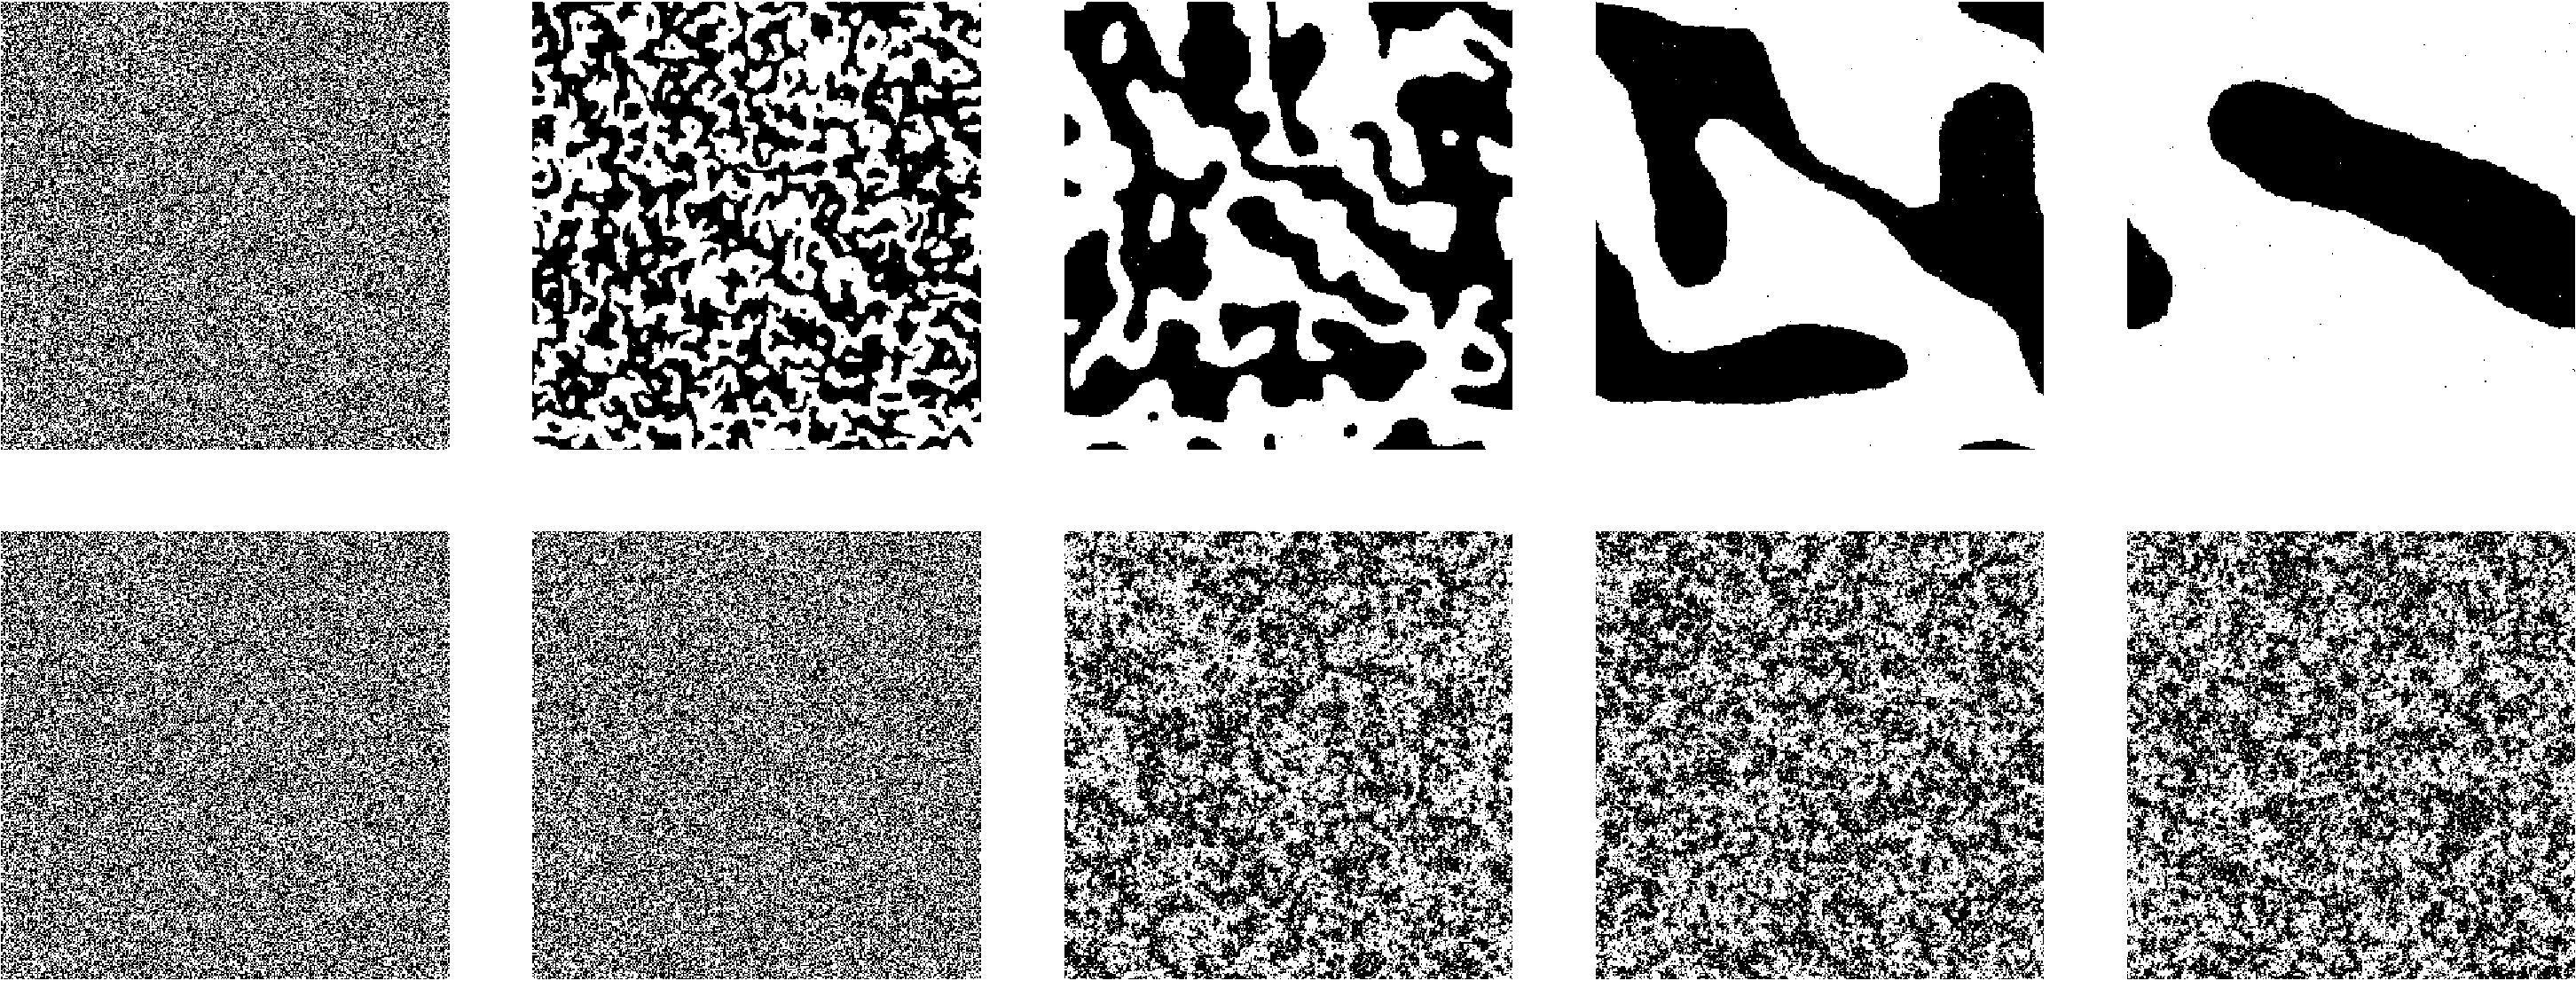
\includegraphics[scale=0.35]{../figures/evolution.pdf}
  \caption{For a $1000\times 1000$ lattice the spin is shown, black is down, white is up, for different MC cycles for two different temperatures. The top row is for a temperature of $1.0J/k_B$, and the bottom row is for a temperature of $2.4J/k_B$; one on each side of the critical temperature. For each temperature the spins are shown after different number of MC cycles, from left to right we have shown the spins after $0$, $10^2$, $10^3$, $10^4$ and $10^5$ MC cycles. The initial state for both temperatures was chosen to be random.}
  \label{fig:evolution}
\end{figure*}
\subsection{Units}
In our simulations we will scale the equations by using natural units of $J$ and $k_B$. This way our results are on the order of $1$, and we will avoid overflow or underflow errors due to the size of the numbers. By using these natural units we will find the answers in units relevant for our system. For example will the unit of energy be $J$, the unit of heat capacity be $k_B$, the temperature be $J/k_B$ and the unit of magnetic susceptibility be $1/J$. We will use this as the unit for all of our results. \\
In our results we will always show each property as per particle. This way we can easily compare results for different lattice sizes, since it is the, for example, energy per spin, we are studying.\\Since the spin and expectation values always are integers, we will save the variables as integers to reduce the computation time of our algorithm.

\subsection{Parallelization}
As we want to find the expectation values for many temperatures we should minimize the run time of our algorithm. One step to do this is to parallelize. This way we distribute the work to four different cores. This is implemented by letting each core calculate one forth of the algorithm each. Each core calculates a set of temperatures for every lattice size, and writes the results to file. Since this activity is separate from each other, all cores can work simultaneously on the same problem. When we want to analyze the result we just have to read the data files which each core produced. We ran on four cores on two different computers, meaning that we ran on eight cores. This made it possible to do the calculation for many values of the temperature, and to have large lattice sizes.

\section{Results}

\subsection{Testing with theory}
To make sure our algorithm is correct we start by simulating for a $2\times 2$ lattice. For this system we have analytical expressions for the expectation values, see section \vref{sec:analytic}. We calculate the expectation values for temperatures between $0.5$ and $4$, using $10^{6}$ MC cycles. This produces the results shown in figure \vref{fig:2times2}.

\subsection{Reaching equilibrium}
To find how many MC cycles are needed to reach equilibrium we plot the expectation value of the energy and absolute magnetization as a function of MC cycles. We get information about the transition to equilibrium for different initial conditions, and different temperatures; one temperature above the critical temperature, and one below. This is done for one ordered initial condition, all spins pointing up, and one disordered, the spin direction is chosen randomly for each spin. This is shown for the energy in figure \vref{fig:problem_c_E} and for the magnetization in figure \vref{fig:problem_c_M}. These two plots give us information about how many MC cycles are need to reach equilibrium. After around $10^4$ MC cycles the expectation values are close to equilibrium, and after $10^5$ it is constant.

\begin{figure*}
\centering
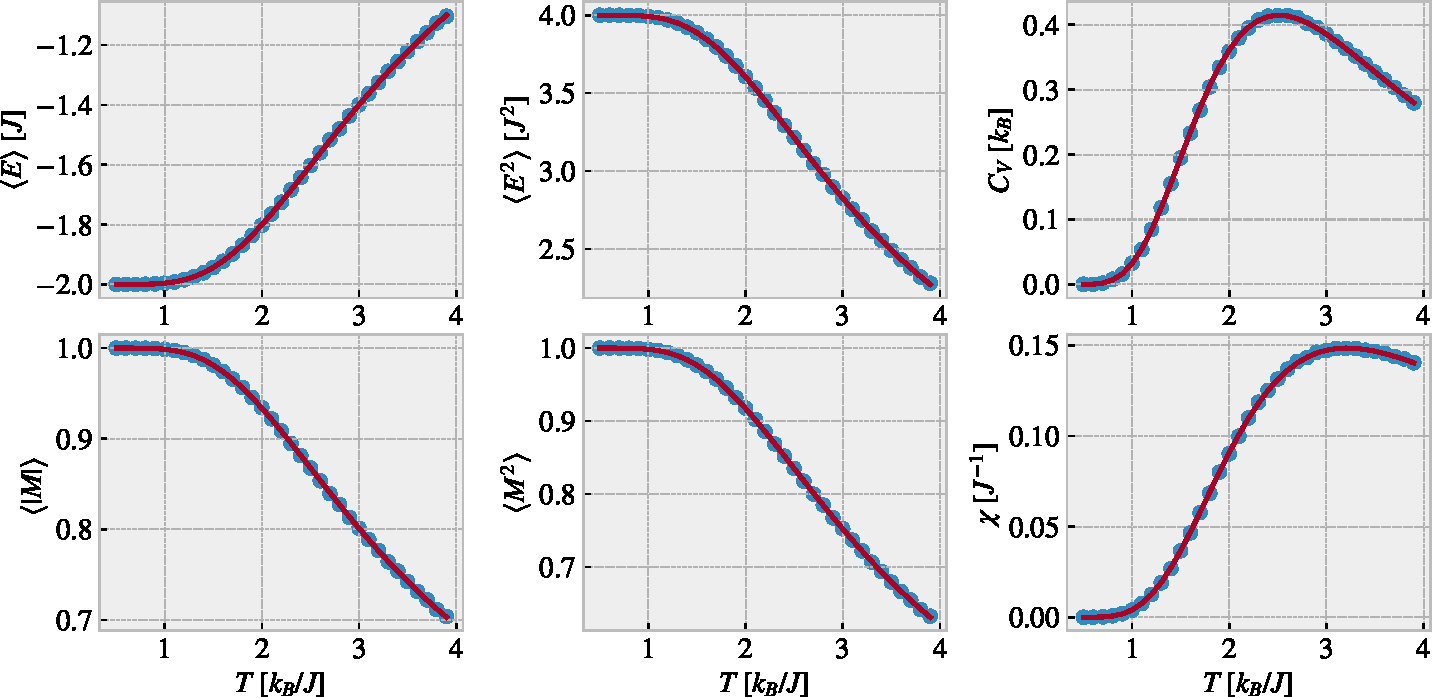
\includegraphics[width=0.9\textwidth]{../figures/taskb.pdf}
\caption{Numerical value and theoretical value of energy, energy squared, absolute magnetization, magnetization squared, heat capacity and magnetic susceptibility. The blue dots are the measured numerical values, and the red line is the analytical prediction. This was calculated for a $2\times 2$ system with $10^6$ Monte Carlo cycles. This was made with a change in temperature of $0.1$. The $x$-axis is the same for all $6$ figures. The analytical expressions for the expectation values are described in section \vref{sec:analytic}.}
\label{fig:2times2}
\end{figure*}
\begin{figure}
  \centering
  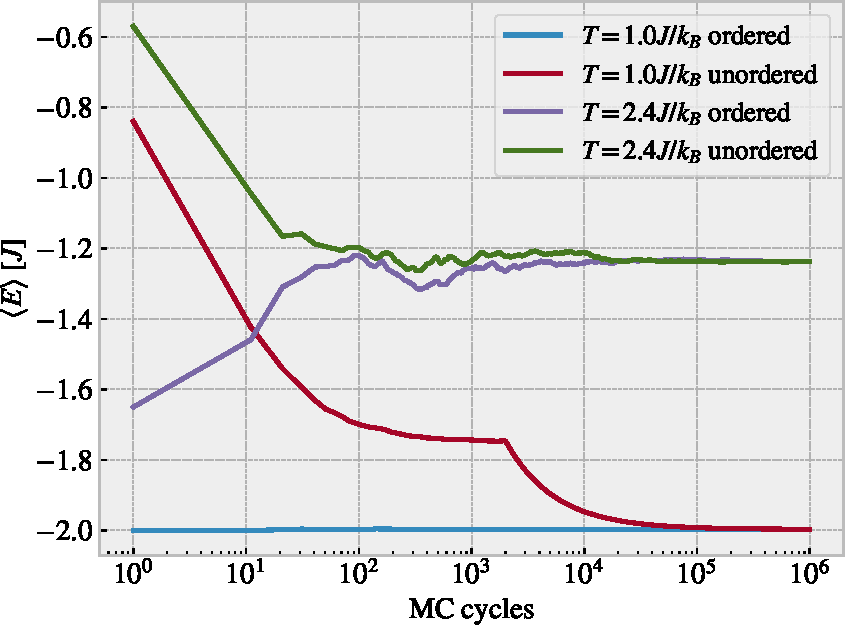
\includegraphics[width=0.5\textwidth]{../figures/problem_c_E.pdf}
  \caption{The expectation value of the energy as a function of MC cycles for a $20\times 20$ lattice with two different initial conditions with two different temperatures. The ordered state means that the initial state was all spins pointing up. The disorder state means each spin was chosen, with equal probability, either up or down. One temperature is above the critical temperature, and one is below.}
  \label{fig:problem_c_E}
\end{figure}

\begin{figure}
  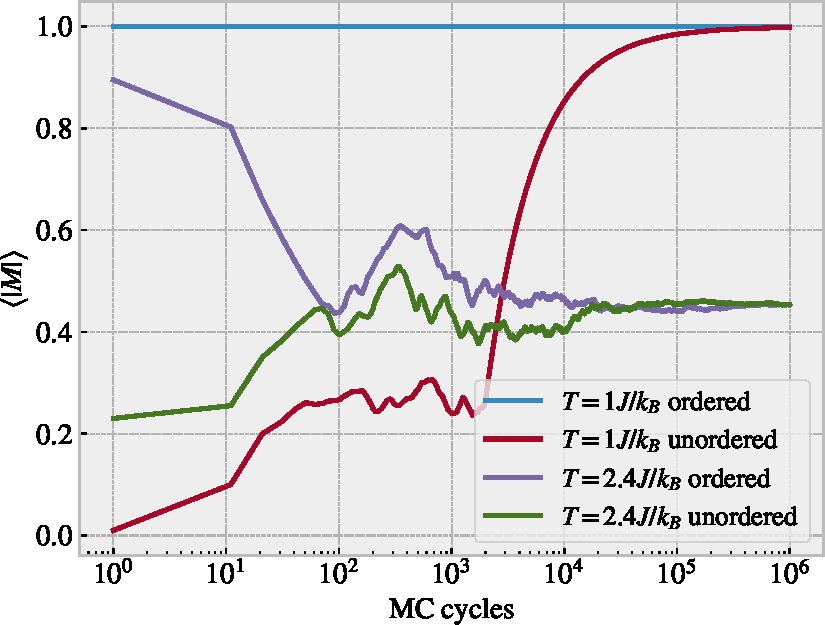
\includegraphics[width=0.485\textwidth]{../figures/problem_c_M.pdf}
  \caption{The expectation value of the absolute magnetization as a function of MC cycles for a $20\times 20$ lattice with two different initial conditions with two different temperatures. The ordered state means that the initial state was all spins pointing up. The disorder state means each spin was chosen, with equal probability, either up or down. One temperature is above the critical temperature, and one is below.}
  \label{fig:problem_c_M}
\end{figure}

In addition we want to find the percent of accepted flips as a function of number temperature. This is shown in figure \vref{fig:problem_c_accept} for a $20\times 20$ lattice with temperatures between $0.2J/k_B$ and $4.8J/k_B$.

\begin{figure}
  \centering
  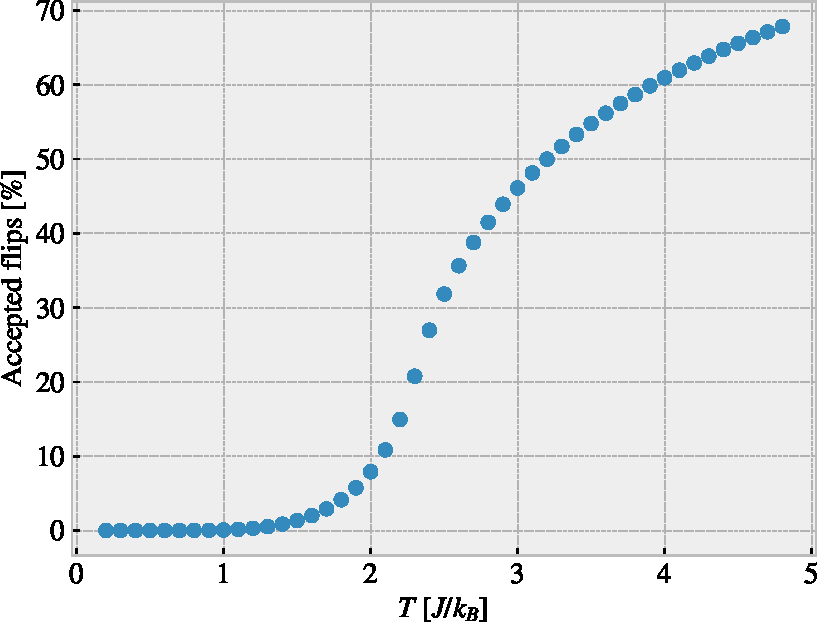
\includegraphics[width=0.485\textwidth]{../figures/problem_c_2.pdf}
  \caption{The percent of accepted flips after $10^6$ MC cycles as a function of temperature for a $20\times 20$ lattice. The temperatures was chosen to see the the percent accepted flips below and above the critical temperature. The flips was counted $L^2$ times for each MC cycle, resulting in a maximal number of flips equal to $4\times 10^8$, the percent is only calculated after all MC cycles. The number of accepted flips is including the equilibration flips, where the initial state was random for all temperatures.}
  \label{fig:problem_c_accept}
\end{figure}



In figure \vref{fig:evolution} we have displayed the spin structure for temperatures $1J/k_B$ and $2.4J/k_B$ to visualize the path from the initial state to the equilibrium state as a function of MC cycles, with black being down, and white being up, for a $1000\times 1000$ lattice.

\subsection{Probability distribution function}
In figure \vref{fig:problem_d} we have shown a histogram of each time an energy occurs for a $20\times 20$ lattice, with a temperature of $1.0J/k_B$ and $2.4J/k_B$ over $10^6$ MC cycles. For $T=1$ we find that the average energy is $-2.00$ with a variance of $0.01$. While for $T=2.4$ the average energy is $-1.25$ with a variance of $0.14$.

\begin{figure}
  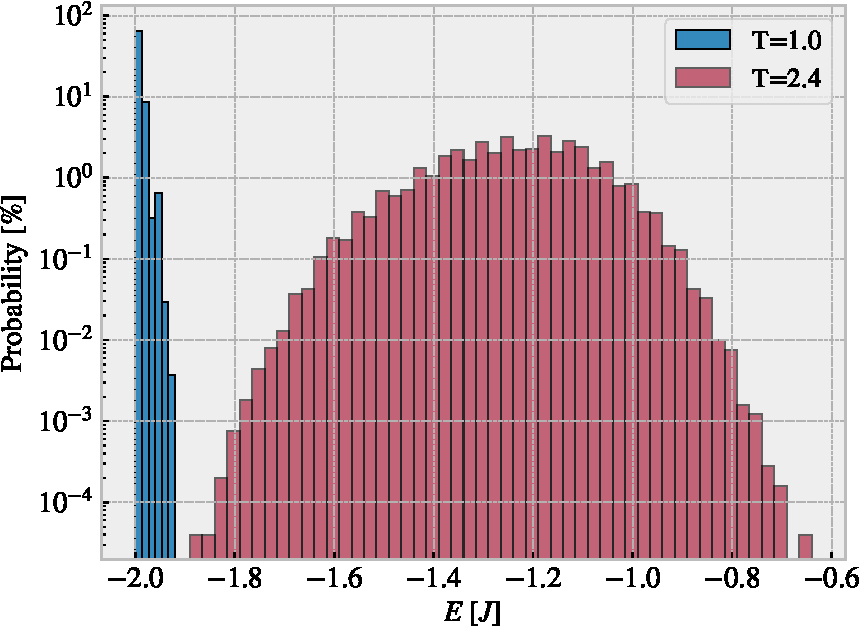
\includegraphics[width=0.485\textwidth]{../figures/problem_d.pdf}
  \caption{Number of occurrences of a given energy for a $20\times 20$ lattice with two different temperatures $1.0J/k_B$ and $2.4J/k_B$ for $10^6$ MC cycles. This is plotted with a logarithmic $y$-axis with $5$ bins for the lower temperature, and $50$ bins for higher temperature.}
  \label{fig:problem_d}
\end{figure}

\subsection{Parallelization}
Since we want to run for large lattice sizes the code is ran in parallel on four cores. We performed a timing of the code with and without parallelization. The resulting time is shown in figure \vref{fig:timer} for different lattice sizes, where we timed the code when it had to calculate the first $10^5$ MC cycles for eight different temperatures, for each lattice size. The same data shown in the figure was used to calculate other properties. In a log-log plot we find that the un-parallelized code has a slope of $1.996(4)$, and the parallelized code has a slope of $1.90(5)$. When calculating the relationship of the two, we find that the parallelized code runs $3.6(2)$ times faster than the un-parallelized code.

\begin{figure}
  \centering
  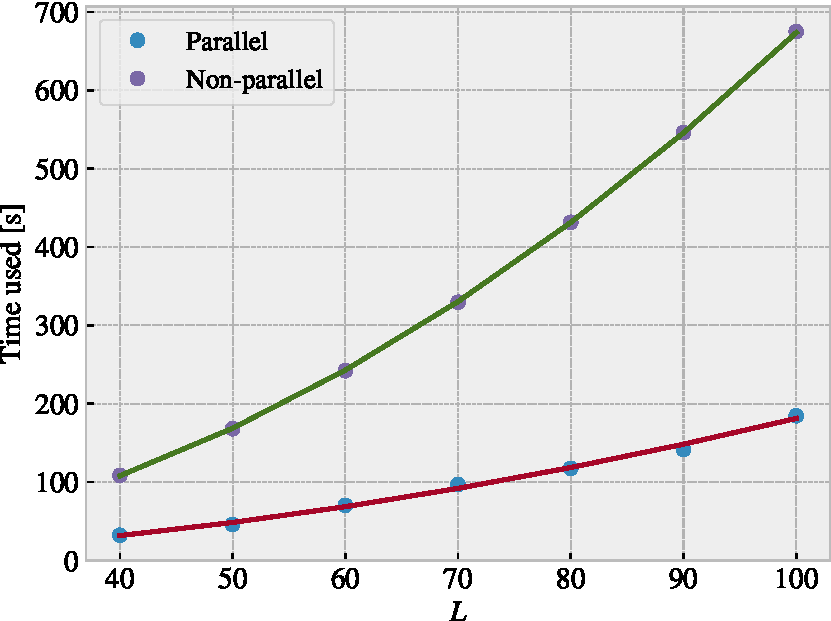
\includegraphics[width=0.485\textwidth]{../figures/timer.pdf}
  \caption{A timing of the algorithm was produced for different lattice size to display the run time dependency on the lattice size with and without parallelization on four cores. Each dot represents a timing, and the curves represent the best fit using the least squares method \cite{squires}. The time used for each lattice size is to calculate the first $10^5$ MC cycles for eight different temperatures.}
  \label{fig:timer}
\end{figure}

\subsection{The phase transition}
To study the phase transition we calculate the expectation values for temperatures around the critical temperature. We do this for different lattice sizes $40, 60, 80$, $100$, $120$ and $200$. We calculated the expectation values with a step of $0.01J/k_B$, but decreased the step to $0.0025J/k_B$ around the critical temperature. From these expectation values we can calculate the heat capacity \eqref{eq:Cv} and magnetic susceptibility \eqref{eq:chi}.
In figure \vref{fig:task_e_absM} the absolute magnetization is displayed as a function of temperature for different lattice sizes, and the same in figure \vref{fig:task_e_E} for the energy. In figure \vref{fig:heat_cap} the heat capacity is displayed and in figure \vref{fig:chi} the magnetic susceptibility, both as a function of temperature. In figure \vref{fig:heat_cap_fit} the heat capacity is displayed more accurately around the critical temperature, with it's best fit lines using the Savitzky–Golay filter.\\


\begin{figure}
  \centering
  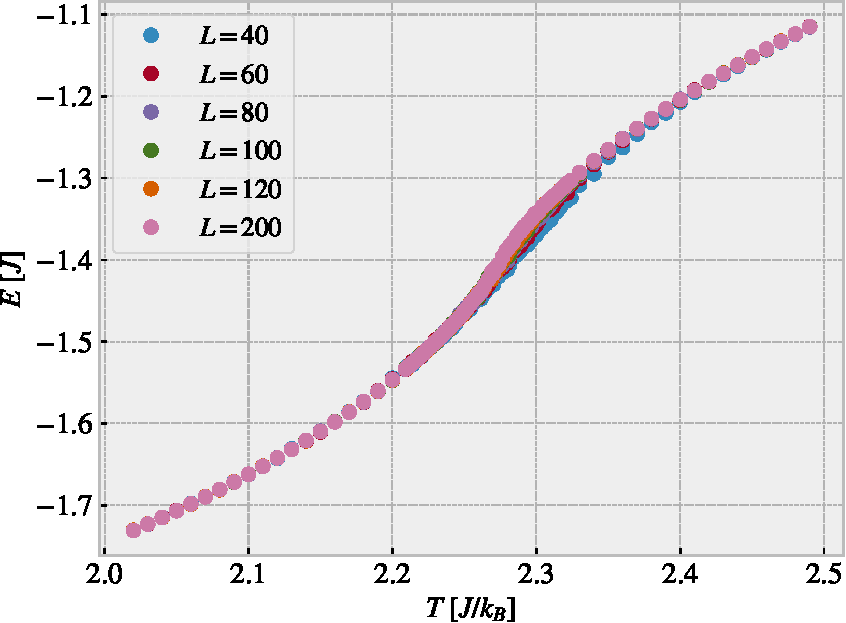
\includegraphics[width=0.485\textwidth]{../figures/energy.pdf}
  \caption{The energy per spin as a function of temperature for different lattice sizes $L$. The energy per particle is displayed around the critical temperature to study the phase transition. By showing for different lattice sizes we can see how the phase transition depends on the lattice size.}
  \label{fig:task_e_E}
\end{figure}

\begin{figure}
  \centering
  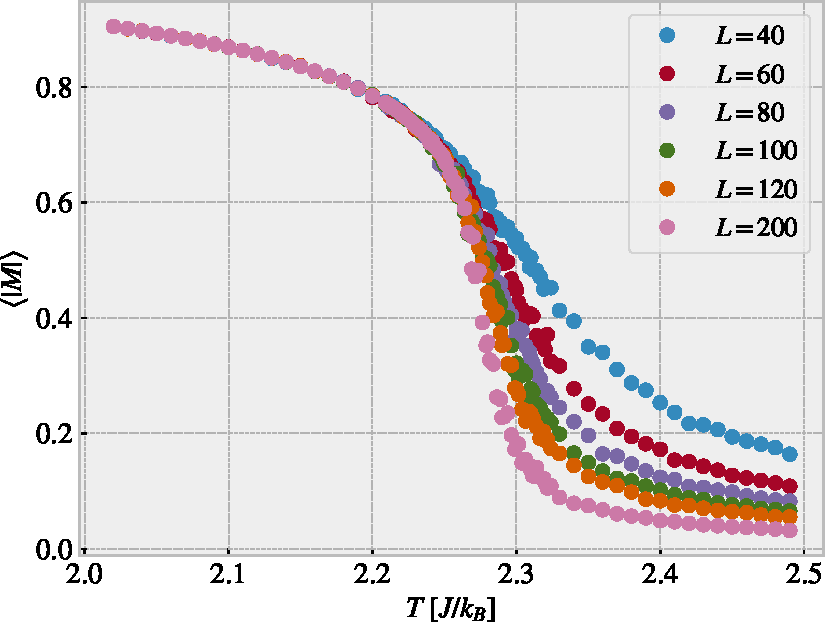
\includegraphics[width=0.485\textwidth]{../figures/magne.pdf}
  \caption{The absolute value of the magnetization $\langle \abs{M} \rangle $ as a function of temperature for different lattice sizes $L$ is displayed around the critical temperature to study the phase transition. By showing for different lattice sizes we can see how the phase transition depends on the lattice size.}
  \label{fig:task_e_absM}
\end{figure}

\begin{figure}
  %\centering
  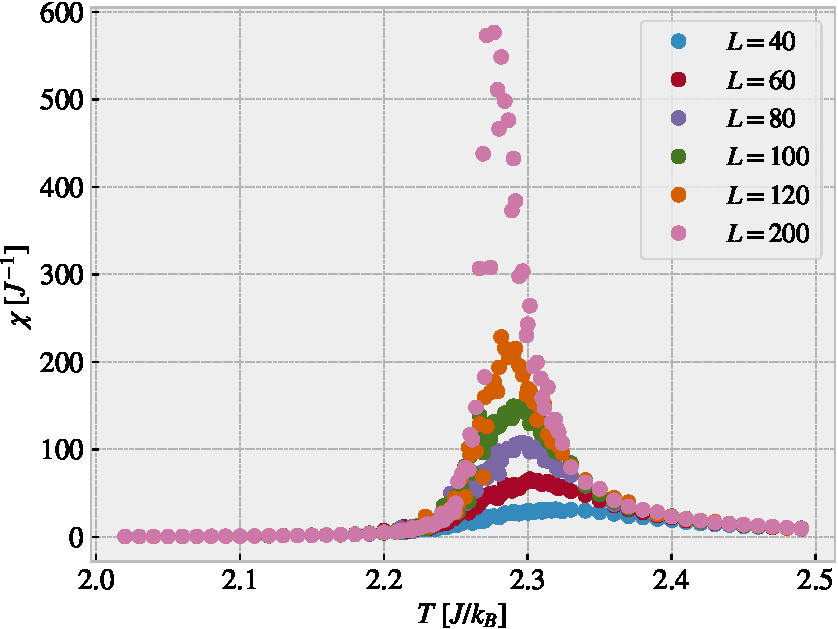
\includegraphics[width=0.485\textwidth]{../figures/suscept.pdf}
  \caption{The magnetic susceptibility $\chi$ \eqref{eq:chi} as a function of temperature for different lattice sizes $L$. The magnetic susceptibility is displayed around the critical temperature to study the phase transition. By showing for different lattice sizes we can see how the phase transition depends on the lattice size.}  \label{fig:chi}
\end{figure}

\begin{figure}
  \centering
  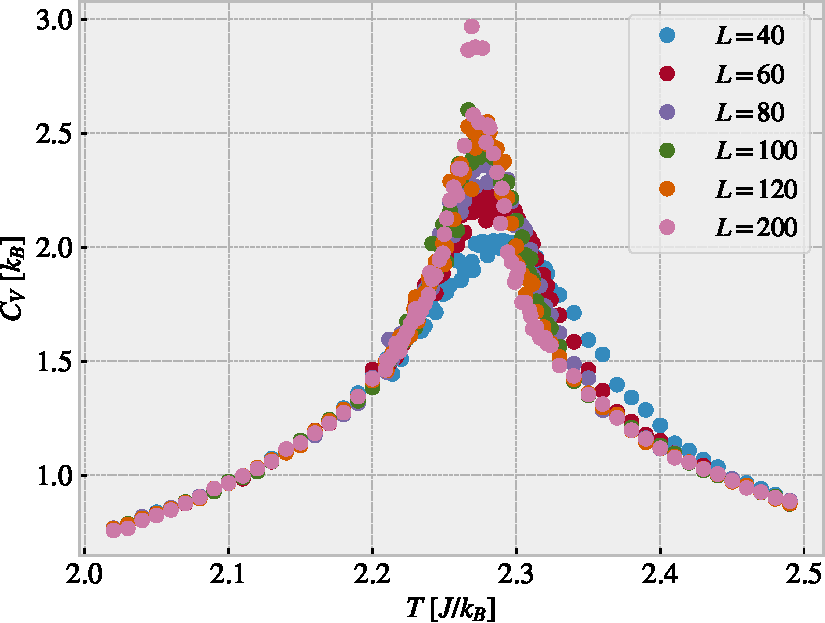
\includegraphics[width=0.485\textwidth]{../figures/heatcap.pdf}
  \caption{The heat capacity $C_V$ \eqref{eq:Cv} as a function of temperature for different lattice sizes $L$. The heat capacity is displayed around the critical temperature to study the phase transition. By showing for different lattice sizes we can see how the phase transition depends on the lattice size.}
  \label{fig:heat_cap}
\end{figure}

\begin{figure}
  \centering
  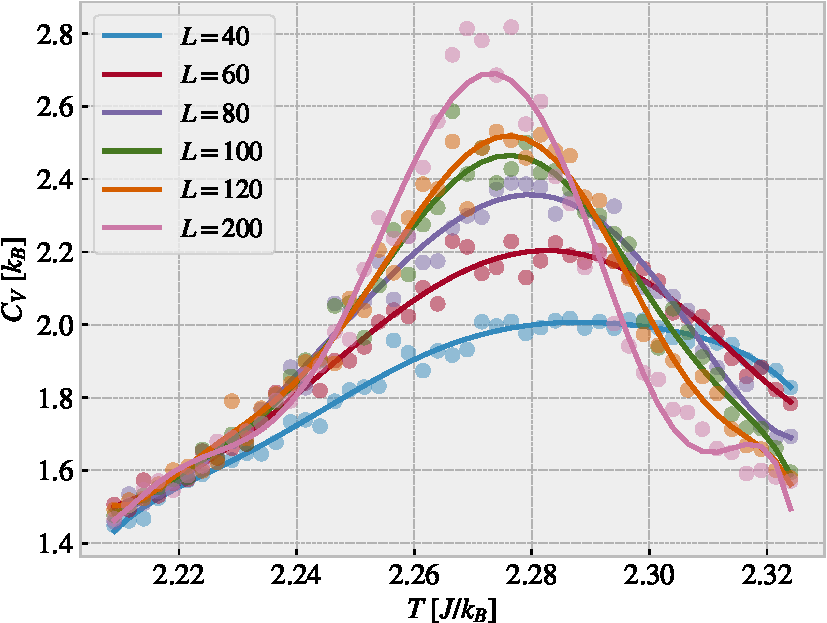
\includegraphics[width=0.485\textwidth]{../figures/fitted_suscept.pdf}
  \caption{The heat capacity $C_V$ \eqref{eq:Cv} as a function of temperature for different lattice sizes $L$. The heat capacity is displayed around the critical temperature to study the phase transition. By showing for different lattice sizes we can see how the phase transition depends on the lattice size. The best fit lines are chosen using a Savitzky–Golay filter.}
  \label{fig:heat_cap_fit}
\end{figure}

From theory the critical temperature is at the temperature corresponding to the maximum value of the heat capacity and the magnetic susceptibility. From the data shown from figure \vref{fig:heat_cap_fit} we can estimate the critical temperature using equation \eqref{eq:noe}, the result of this calculation is displayed in figure \vref{fig:find_Tc}.

\begin{figure}
  \centering
  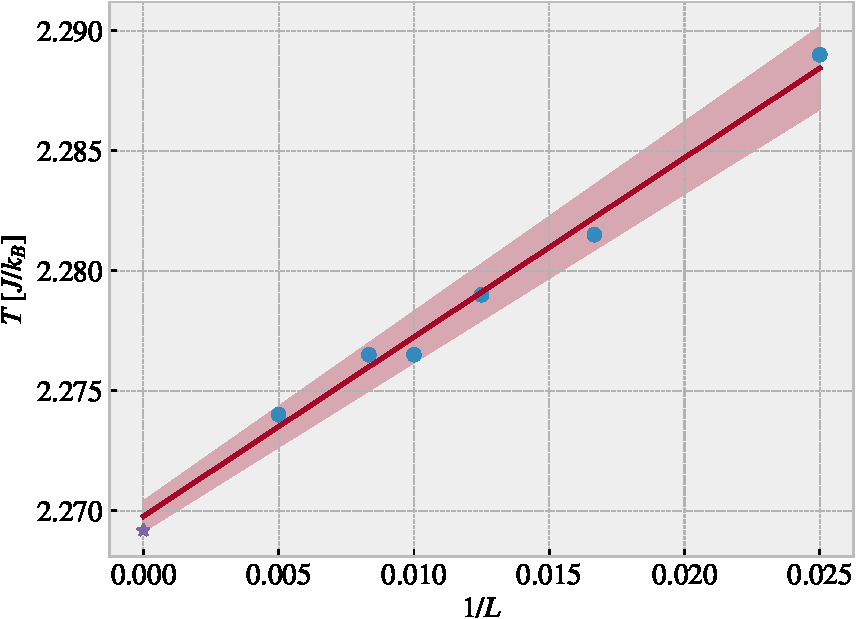
\includegraphics[width=0.485\textwidth]{../figures/TC.pdf}
  \caption{The temperature value corresponding to maximal value of the heat capacity is shown as function of the reciprocal lattice size. The temperature corresponding to maximal heat capacity was chosen using Savitzky–Golay filter on the heat capacity for each lattice size. Using a linear regression \cite{squires} on this data we find the result of the critical temperature on the form of equation \eqref{eq:noe}, which we use to find the critical temperature for $L=\infty$, by finding the best fit line's value for $1/L=0$. The star shows the analytical value of the critical temperature, and the read area shows the uncertainty of the linear regression.}
  \label{fig:find_Tc}
\end{figure}


\section{Discussion}
\subsection{Testing with theory}
From figure \vref{fig:2times2} we see that our algorithm produce the correct results for the $2\times 2$ system. The analytical results we tested against is described in section \vref{sec:analytic}. As this was calculated for a small system, we should not focus too much on the behaviour of the different physical properties for different temperatures, especially around the critical temperature. The important result from this figure is that our algorithm is able to reproduce the analytic result to great accuracy. By changing a single variable we can increase the size of our system, and our results will then most likely be correct for larger, more complex system. To get expectation values consistent with theory we need to use $10^5$ MC cycles. This was found by running the code for different number of MC cycles and analyzing the result.
\subsection{Reaching equilibrium}
The expectation value for different MC cycles is studied closer in figure \ref{fig:problem_c_E} and \vref{fig:problem_c_M}, where we have displayed how the system reaches it's equilibrium for different initial conditions for different temperatures.
For the low temperature, we see that the equilibrium state is almost instantaneously reached for the order initial condition, with no fluctuations. While the disordered initial condition needs around $10^4-10^5$ MC cycles for equilibrium to be reached. This is due to the Ising model having an ordered, low entropy system, under the critical temperature, where the spins want to align. When every spin is pointing the same direction any flip of a spin results in a change of energy equal to  $8J$. This makes the change in energy always positive, and the spin will never be flipped due to the first requirement in the metropolis algorithm. The second requirement, with the relative Boltzmann factor \eqref{eq:prob_rel}, is not possible either, as it is too small for the randomly generated number $r$ between zero and one to be smaller. Therefore the ordered initial condition will already be in it's equilibrium state, and equilibrium is reached instantaneously. The extremely low probability of flipping as spin makes the equilibrium state very stable, as we can see in the two figures. \\
For the higher temperature system the equilibrium state is fluctuating more than the ordered state. Due to the equilibrium state being $50\%$ pointing up, and $50\%$ pointing down, the change in energy when flipping a spin can take on any value, both positive and negative. This makes the first requirement of the metropolis algorithm, occur much more often than in the ordered state. If not, the Boltzmann factor \eqref{eq:prob_rel} is much smaller, due to the value of $\beta$ being smaller, which will make the probability of flipping a spin much larger than for the $T=1$ system.\\
For the higher temperature we see that both the ordered and disordered state uses around the same number of MC cycles to reach the equilibrium state. For this temperature the equilibrium state is quite close to the average of the two different initial states. This makes the number of MC cycles needed for equilibrium around $10^4$.\\
From this result we can estimate an equilibrium time for our system. We find the number of MC cycles needed to reach equilibrium for this lattice size $L=20$, and for these two temperatures. As the number of randomly selected spins scales with $L$, the size of the system should not change the equilibration time. We interestingly find that the pick of initial state does not effect the equilibration time any large amount. To be sure that the system has reached a very stable equilibrium we should use around than $10^5$ MC cycles.\\
Our results indicate that the equilibration time is independent of initial condition, and temperature. The results was only calculated for a $20\times 20$ lattice, but as we choose $L^2$ spins for each MC cycle the size of the system should not effect the equilibration time. We therefore believe that the simple method of running the system for a wanted amount of MC cycles before starting to calculate the expectation values is the optimal method. This is an easy to implement method, guarantees correct results and is easy to combine with using the previous spin configuration when slightly increasing the temperature. A equilibration function which calculates the change in a for example the absolute magnetization to find the equilibrium state can be implemented in a way which makes it requirement to strict for some temperatures and lattice sizes, and too tolerant for others. Setting a fixed amount of MC cycles also makes the run time of the algorithm known, as the number of MC cycles is known. This is not guaranteed with the other method. \\
The reason for the system not starting ordered in the figure is that we do not write every spin state to file, and the initial state is therefore not displayed.\\
As the state with unordered initial spins is approaching it's equilibrium value we observe an exponential approach towards the end, for both energy and magnetization, what is the reason behind this behavior? As the system is approaching it's equilibrium there are only a few spins pointing the opposite direction of the others. The fewer spins there are, it is less less likely to select one of the fewer spins. In addition, the fewer spins might be forming an \textit{island}, which makes the spins harder to flip, as they have multiple neighbors with the same spin.
\\In figure \vref{fig:problem_c_accept} the percent of number of accepted spin flips is shown as a function of temperature for a $20\times 20$ system. We see that the number of flips is much lower for the lower temperature states, compared to the high temperature states. For the lower temperatures the percent of accepted flips are around $10^{-5}$, as the temperature approaches the critical temperature the percent increases rapidly. Above the critical temperature it seems like the percentage starts to become saturated, and we are converging to a constant value.

This is due the equilibrium state being different for different temperatures. Below the critical temperature we have an ordered, low entropy, state where flipping a single spin will result in a large increase in energy, making the Boltzmann factors very small, and flipping a spin is improbable. Above the critical temperature the spins are equally distributed, this gives the change in energy the possibility of taking on all five possibilities. We will therefore continue to flip spins in the high temperature limit. This makes the actual percentages dependent on the number of MC cycles, as the equilibration flips will play a smaller and smaller role of the total amount of flips as we increase the number of MC cycles.\\
The fact that the equilibrium state is different for the two systems is clearly displayed in figure \vref{fig:evolution}.
As we are including the equilibration flips we believe the percentage are dependent on the number of MC cycles, as the percent of MC cycles which are for equilibration will effect the final percentage.
\subsection{probability distribution function}
In figure \vref{fig:problem_d} the number of occurrences of a given energy for a $20 \times 20$ system with two different temperatures, $1.0J/k_B$ and $2.4J/k_B$ is shown. From this data we find the probability distribution function for the two functions, without ever having to calculate it. We see that for the low temperature, below the critical value, the distribution function is very narrow, with almost all energies being of the same value. While for the higher temperature, above the critical value,  there is a large spread in the different energy values. This is consistent with the results we have discussed earlier. For the lower temperature the equilibrium state has a  very low probability of flipping a spin, resulting in the same energy occurring many times. While for the higher temperature we keep flipping spins, resulting in different energies. The main difference of the two probability distributions, other than their average, is their variance. Which we calculated to be $0.008J/k_B$ and $0.147J/k_B$ for temperatures of $1J/k_B$ and $2.4J/k_B$ respectively. For the higher temperature the variance is a factor of $18.4$ larger, displaying many more accessible states around the stable equilibrium, we have larger fluctuations. This is consistent with what we have observed previously, there are more different accessible states, more change, in the high temperature and entropy system, compared to the lower energy and entropy system, where a change of a single spin will result in a large change in energy.
\subsection{Parallelization}
In figure \vref{fig:timer} the time used is displayed with and without parallelization for different lattice sizes. As the code uses a long time to run for large lattice sizes it was necessary to parallelize the code. The process which was needed to calculate was $10^5$ Monte Carlo cycles for eight different temperatures. By calculating the slop in a log-log plot the un-parallelized code had a slope of $1.996(4)$, meaning that the time scales as $L^2$. The parallelized code has a slope of $1.90(5)$ in a log-log plot, meaning that that the time used scales as $L^{1.90}$. The two methods has approximately the same slope, but has a much different constant term in the log-log plot. This difference in constant term is enough to make the parallelized code $3.6(2)$ times faster than the un-parallelized code. As we are calculating the time for eight different temperatures, and the work was distributed on four cores, it makes sense that the time is almost a factor of four less. The reason for why it is not exactly $4.0$ is probably due to the code having to distribute and set up the parallelization for each lattice size. \\
We also notice that the code is inefficient, as it takes more than $11$ minutes to calculate eight temperatures for the $100\times 100$ lattice without parallelization. While for a parallel run it takes a little over $3$ minutes, a huge difference in computational time. This is the reason for why the code was parallelized.
\subsection{The phase transition}
In figure \ref{fig:heat_cap} and \vref{fig:chi} the heat capacity and magnetic susceptibility is displayed accordingly. For both of these properties we see a maximum value around the critical temperature. At the maximum value we are at the phase transition of the system. Theoretically both of these values should diverge (\ref{CVALPHA},\ref{CHIGAMMA}), but is not something we will observe numerically. We will only find a larger and narrower spike as we increase the lattice size, and are approaching the thermodynamic limit. We see a similar behaviour for the absolute magnetization, shown in figure \vref{fig:task_e_absM}. Where we theoretically expect zero absolute magnetization after the critical temperature, but our system is instead approaching zero slowly. How fast the system is approaching zero is dependent on the lattice size, and we see that the larger system is approaching zero faster. The reason we expect zero is that for the high entropy system we should have equal amount pointing up as down. We have observed that the model exhibits a phase transition from a magnetic phase (a system with a finite magnetic moment) to a phase with zero magnetization.\\
From the data we can clearly see that as we increase the size of the system, the closer we will come to the analytical value of the phase transition. This is due to the analytical values being true in the thermodynamic limit. If we were to simulate for larger systems, we would approach the analytical value even closer. As the size of the system is increased, the boundary effects become vanishingly small.\\
For the energy, shown in figure \vref{fig:task_e_E}, there is no abrupt change around the critical value, and there is little change when increasing the system size. What we observe is a weak splitting of energy after the critical temperature. Where the larger system size increases it's energy by more than the smaller systems, deviating from their linear dependence on temperature. While for temperatures above the critical temperature we see that the lattice size no longer effects the energy, and we find the same value for different lattice sizes. A reason for this change might be the displayed in the heat capacity, shown in figure \vref{fig:heat_cap}. The heat capacity tells us the change in energy due to changes in temperature, and we see that the values of the heat capacity is strongly dependent on lattice size. For larger lattices the change in energy when increasing the temperature is larger, this makes the energy per particle larger for larger lattices, which is what we observe. In addition we see that the heat capacity for large lattice sizes are lower above the critical temperature, thus giving making the energy the same, independent of lattice size, for higher temperatures.\\
In figure \vref{fig:find_Tc} we have used the critical temperature found numerically together with equation \eqref{eq:noe}, as a function of the reciprocal lattice size. To extract the critical temperature more accurately we used a Savitzky–Golay filter, and found the temperature resulting in the largest heat capacity of the filtered data, this is shown in figure \vref{fig:heat_cap_fit}. By using the least squares method to find the best fit line, and evaluating it at $1/L=0$, we get a critical temperature extremely close to the analytical, where we found a value of $2.2698(6)J/k_B$, when the analytical value is $ 2.2692J/k_B$. Our resulting temperature is consistent to the analytical within uncertainties. We have a large uncertainty in our results, which comes from the uncertainty in the least squares method \cite{squires}. There are other uncertainties, which is not accounted for, in the selection of the critical temperature for each lattice size, which would make the uncertainty.

\section{Conclusion}
The Ising model is studied using the Monte Carlo based Metropolis algorithm numerically in a two dimensional lattice with periodic boundary conditions. We start with simulating the $2\times 2$ lattice and comparing our results with the analytical ones. We find that our numerical results fit perfectly with the analytical result. For the results to match theory we see that we need $10^5$ MC cycles.\\
In our code we can easily expand the size of the lattice by increasing a single variable, we start by analyzing the $20\times 20$ lattice. Here we studied the Monte Carlo cycles path to equilibrium for different temperatures and different initial conditions. We saw that it is generally needed more than $10^4$ MC cycles before reaching equilibrium. For low temperature system equilibrium is reached much faster with an ordered state, for higher temperature both ordered and disordered state reach equilibrium around the same time. From the results we see that the values are fluctuating around equilibrium, which is a high entropy state. For the low temperature, low entropy state, we see very small fluctuations. Calculating the probability distribution function is numerically impossible for large system, but by making a histogram of when energies occurs we can find the probability distribution function without ever having to calculate it. Parallelizing the code on four cores make the runtime of the algorithm increase by a factor of $3.6$. By studying macroscopic properties around the phase transition we are able to find the critical temperature of the Ising model, $2.2698(6)J/k_B$, when the analytical value is $ 2.2692J/k_B$, correct to the analytical one within uncertainties.

\section{Comments}
All of the code used is available on my GitHub (\url{http://www.github.uio.no/ivarsh/FYS4150}). Here the \texttt{README.MD} files will describe the structure of our GitHub, and the purpose of each program. The code itself will also include notes explaining what it does.

\bibliography{citations.bib}{}
\bibliographystyle{plain}


\end{document}
